\chapter{Introduction}
\label{introduction}



\begin{center}
  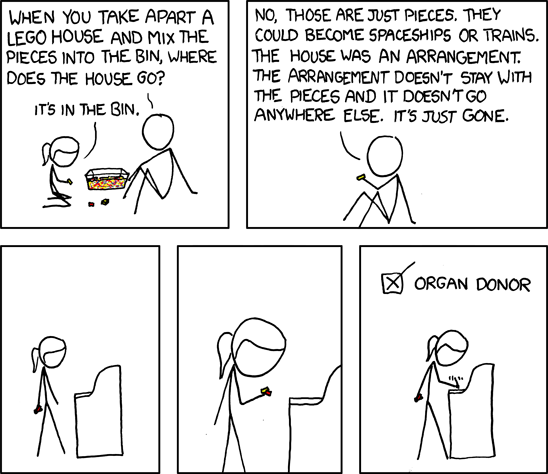
\includegraphics[width=9cm]{introductionpics/lego}
\end{center}
\textit{XKCD Lego}


%\begin{quotation}
%\textbf{Man}: When you take apart a Lego house and mix the pieces into the bin, where does the house go?\\
%\textbf{Woman}: It's in the bin.\\
%\textbf{Man}: No, those are just pieces. They could become spaceships or trains. 
%The house was just an arrangement. The arrangement doesn't stay with the pieces and it doesn't go anywhere else. It's just gone\\
%--XKCD Lego
%\end{quotation}

%%%The start of this thesis leads the reader to the idea that when building a complex system, breaking the probelm into parts is a natural and beneficial instinct\\
{}When confronted with building a complex system, our first instinct in an attempt to construct the system is often to break it into smaller, simpler components. 
{}These are defined by their contribution to the system and their relationships to other components.
{}Through this ``divide and conquer'' method, the design and construction of a complex system becomes a manageable task.

%%%We use the metaphor of building a car to explain the benefits of breaking systems into components
When building a complex system like a car, you would not attempt to build the car as a whole, but break it into parts for design and construction.
A car requires a body, electrical system, interior, suspension and steering, engine \ldots. 
The engine can be further broken into other parts like cooling, oil system, exhaust and intake systems, fuel, and so on.
Each of these parts have relationships that lead to complex dependencies; for instance, the \textit{carburettor} blends the air from the \textit{intake} with petrol from the \textit{fuel system}.

%%%The benefits of breaking apart systems are gained during design, implementation, maintenance and evolution. 
The benefits of breaking a system apart are gained through the entire product process; design, implementation, deployment, maintenance and evolution.

%%%During Design; more informed planning, understanding the "big picture", risk analysis

%%%During implementation; specialization of people to tasks, concurent development, testing each part separtly, risk mitigation (if an individual component fails, the entire system is salvageable)

%%%During maintenance; a component can be replace with known side effects, problems can be detected and solved.
The apocryphal story of George Washington's axe which has three times had its handle replaces and twice its head replaced deomstrates the power of maintence on a system of parts.

%%%During Evolution; replacing a component with a superior part, extra components can be added to improve and add functionality.

\section{Software Components}
{}The use of components in software systems has additional benefits over their use in physical systems.
{}Software components can be reused in different contexts, replaced ``on the fly" without interruption to the system, validated for correctness before being used, 
{}and automatically composed into a system through resolving their defined dependencies.

%%%A software component can provide its services to many other components all for different purposes.
In a physical car there are pumps which accomplish many different tasks, pumping oil, air, water.
In a software system such replication is unnecessary as a single component could provide a service that pumps, 
and other components can use this service for many different purposes.
A software component, not bound by physical limitations, can be in many places at once, doing many similar jobs simultaneously.
A component providing a http server can be used for web site hosting, communication, internal and external web-sites, REST and SOAP communication.
This is done all by the same component, as the abstraction of the http service is broad enough to accomplish many tasks.

%%%Changing components while the system is running is possible in software.
Replacing a tire or repairing a windshield while continuing to drive the car is at the very least difficult, if not impossible.
Inside a software system, where changes in state are accomplished so quickly that they are unperceivable, the replacement of parts of a system are easily accomplished while the system is running.

%%%If the software component relationships are well defined, with contracts and requirements a system or component can be validated to be correct before use (e.g. treaty)
If an enthusiast adds a turbo to a car, it may not work correctly in that context, it may create too much pressure and blow the engine.
A component can have complex mechanisms like contracts or strictly defined specifications to automatically detect these incompatibilities before they cause problems.

%%%Given the relationships in a software component system are strictly defined, we can use these to then find valid combinations with user requirements
Imagine being able to define the car you want by describing the functionality you require, and then a custom car, one that may exist no where else in the world,
is automatically built for you. 
While then driving this car your requirements change, you want to drive off road, then the car changes parts to adapt to your new requirements, new tires, engine, gearbox\ldots
This is the power that dependency resolution offers component systems, automatic resolution of a users requirements.

\section{Research Goals}
{}The aspect of the vast research areas of software components we will look at throughout this thesis is the final point made in the previous section, 
{}the automatic composition of software components through resolving component dependencies.
{}Specifically we will try to answer the question:\\
{}\begin{quote}
%``What effect does using component resolution with different evolution strategies have on component system evolution?''.
{}What are the \textbf{consequences to a component system} while \textbf{optimising for different criteria} during evolution when using \textbf{Component Dependency Resolution (CDR)}?
{}\end{quote}

{}This question leads to three lines of inquiry; component dependency resolution, the optimisation with different criteria, and the consequences of CDR optimisation on component systems.

%%%The questions we aim to answer related to CDR:\\
%%%What is CDR and why use it?; CDR chapter \ref{background}\\
%%%What is necessary of a component model for CDR?; Background chapter \ref{background}\\
%%%How do we formally define CDR?; CDR chapter \ref{cdr}\\
%%%How do we implement CDR?; Implementation chapter \ref{implementation}

%%%The questions we aim to answer related to the optimisation of CDR with different criteria are:\\
%%%How do we represent optimisation in CDR?; CDR chapter \ref{cdr}\\
%%%How do we optimise for criteria?; Implementation chapter \ref{implementation}\\
%%%What criteria are important?; Criteria chapter \ref{criteria}

%%%The questions we aim to answer related to the consequences of such optimisation:\\
%%%What consequences are we looking for?; Criteria chapter \ref{criteria}\\
%%%Are component models  similar enough to generalise our results?; Comparisons chapter \ref{comparison}\\
%%%How can we measure the consequences of criteria?; Simulation chapter \ref{simulation}\\
%%%What are the consequences?; Simulation chapter \ref{simulation}

\section{Thesis Overview}
%%%A list and breif explination of each of the chapters and how they relate to our Research Goals 